\section{Regression Trees}
\label{A:RegTrees}
\textcolor[rgb]{0,0,1}{
In this appendix we explain how Regression Trees are built using an example adapted from~\cite{hastie2009elements}.
Tree-based methods partition the feature space into a set of rectangles (more formally, hyper-rectangles) and then fit a simple model in each one. They are conceptually simple yet powerful.
Let us consider a regression problem with continuous response $\Y = \{Y\}$ and and 2 predictors $\X = \{X_1,X_2\}$, each taking values in the unit interval. The top left plot of Figure~\ref{fig:friedman} shows a partition of the feature space by lines that are parallel to the coordinate axes. In each partition element, we can model $Y$ with a different constant.
\begin{figure}
  \centering
  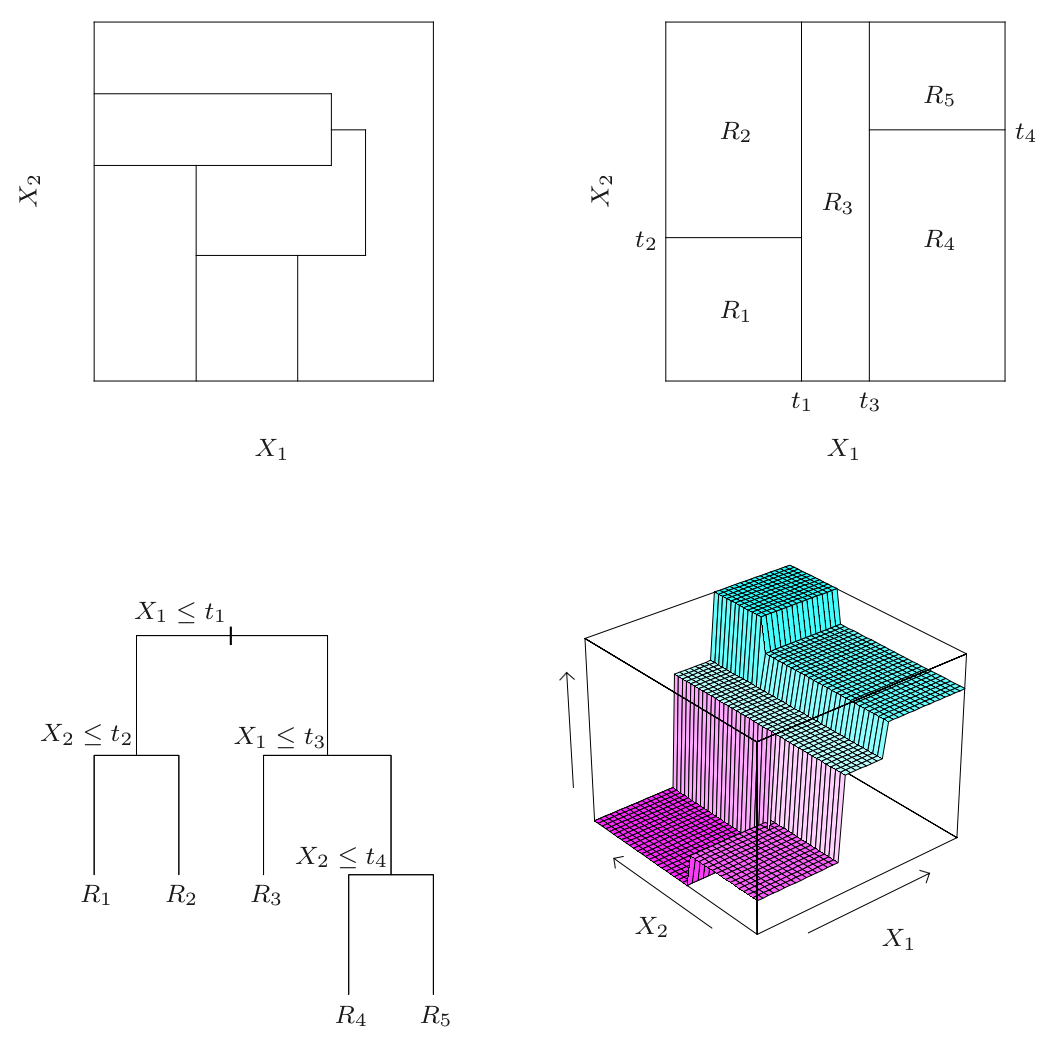
\includegraphics[width=0.7\columnwidth]{figures/friedman.eps}
  \vspace{-8pt}
  \caption{Top right: 2D feature space by recursive binary splitting. Top left: partition that cannot be obtained from recursive binary splitting. Bottom left: tree corresponding to the partition. Bottom right:  perspective plot of the prediction surface.}
  \label{fig:friedman}
   \vspace{-10pt}
\end{figure} 
However, there is a problem: although each partitioning line has a simple description like $X_1 = k$, some of the resulting regions are complicated to describe.
To simplify things, we can restrict ourselves to only consider recursive binary partitions, like the ones shown in the top right plot of Figure~\ref{fig:friedman}.
We first split the space into two regions, and model the response by the mean of $Y$ in each region. 
We choose the variable and split-point to achieve the best prediction for $Y$. 
Then one or both of these regions are split into two more regions, and this process is continued, until some stopping rule is applied. This is the "recursive partitioning" part of the  algorithm. 
For example, in the top right plot of Figure~\ref{fig:friedman}, we first split at $X_1 = t_1$. 
Then the region $X_1 \leq t_1$ is split at $X_2 = t_2$ and the region $X_1 > t_1$ is split at $X_1 = t_3$.
Finally, the region $X_1 > t_3$ is split at $X_2 = t_4$. 
The result of this process is a partition of the data-space into the five regions (or leaves) $R_1, R_2,\cdots, R_5$.
The corresponding regression tree model, $\T$, predicts $Y$ with a constant, $c_i$, in region $R_i$ i.e.,
\begin{equation}
\mathit{f}_{\T}(X_1,X_2) = \sum_{i=1}^{5} c_i I\left\lbrace(X_1,X_2) \in R_i\right\rbrace,
\label{eq:response}
\end{equation}
where $I\{X\in R\}$ is a function that is equal to $1$, if $X\in R$, and $0$, otherwise.
This same model can be represented by the binary tree shown in the bottom left of Figure~\ref{fig:friedman}. 
The full data-set sits at the top of the tree. 
Observations satisfying the condition at each node are assigned to the left branch, and the others to the right branch. The terminal nodes or leaves of the tree correspond to the regions $R_1,R_2,...,R_5$. 
The bottom right plot of Figure~\ref{fig:friedman}, shows the perspective plot of the regression surface obtained as a result of building a regression tree with the 5 constants $c_i,\ i=1,2,3,4,5$. }

\textcolor[rgb]{0,0,1}{
\paragraph{\textbf{Node splitting criteria}}
Now, a first question is: \emph{how to grow a regression tree?}
Suppose our dataset, $(\X,\Y)$, consisting of $p$ features, i.e. $\X = \{X_1,X_2,\ldots,X_p\}$, and one response variable, i.e. $\Y = \{Y\}$. Suppose we have $|(\X,\Y)| = n$ observations (samples): $(x_i,y_i)$, $i=1,2,\ldots,n$, with $x_i=(x_{i1},x_{i2},\ldots,x_{ip})$.
For regression trees we adopt the sum of squares as our splitting criteria, i.e. a variable at a node will be split if it minimizes the following sum of squares between the predicted response and the actual output variable:
\begin{equation}
\sum_i (y_i - \mathit{f}_{\T}(x_i))^2.
\end{equation}
The best response $c_i$ (from equation~\ref{eq:response} for the partition $R_i$), is just the average of output samples in the region $R_i$, i.e.
\begin{equation}
c_i = avg(y_i|x_i \in R_i).
\label{eq:average}
\end{equation}
Finding the best binary partition in terms of minimum sum of squares is generally computationally infeasible. 
A greedy algorithm is used instead. Starting with all of the data, consider a splitting variable $j$ and split point $s$, and define the following pair of left ($R_L$) and right ($R_R$) half-planes
\begin{equation}
\begin{aligned}
R_L(j,s) = \left\lbrace X|X_j \leq s \right\rbrace ,\\
R_R(j,s) = \left\lbrace X|X_j > s \right\rbrace
\end{aligned}
\end{equation}
The splitting variable $j$ and the split point $s$ is obtained by solving the following minimization:
\begin{equation}
\begin{aligned}
\underset{j,s}{\text{min}}\left[\underset{c_L}{\text{min}} \sum_{x_i\in R_L(j,s)} (y_i - c_L)^2 + \underset{c_R}{\text{min}} \sum_{x_i\in R_R(j,s)} (y_i - c_R)^2 \right]  
\end{aligned}
\label{eq:split}
\end{equation}
where, for any choice of $j$ and $s$, the inner minimization in equation~\ref{eq:split} is solved using
\begin{equation}
\begin{aligned}
c_L = \text{avg}(y_i|x_i \in R_L(j,s)),\\
c_R = \text{avg}(y_i|x_i \in R_R(j,s)).
\end{aligned}
\end{equation}
For each splitting variable $X_j$, the determination of the split point $s$ can be done very quickly and hence by scanning through all of the inputs ($X_i$'s), the determination of the best pair $(j, s)$ is feasible.
Having found the best split, we partition the data into the two resulting regions and repeat the splitting process on each of the two regions. Then this process is repeated on all of the resulting regions.}

\textcolor[rgb]{0,0,1}{
Rather than splitting each node into just two regions at each stage, we might consider multiway splits into more than two groups. 
While this can sometimes be useful, it is not a good general strategy. The problem is that multiway splits fragment the data too quickly, leaving insufficient data at the next level down. 
Hence we would want to use such splits only when needed. 
Also multiway splits can be achieved by a series of binary splits.}

\textcolor[rgb]{0,0,1}{
\paragraph{\textbf{Stopping criteria and pruning}}
At this point, the second question is: \emph{How large should we grow the tree?}
Every recursive algorithm needs to know when it's done, i.e. it requires a stopping criteria. 
For regression trees this means when to stop splitting the nodes. 
A very large tree might over fit the data, while a small tree might not capture the important structure.
Tree size is a tuning parameter governing the model’s complexity, and the optimal tree size should be adaptively chosen from the data. 
One approach is to split tree nodes only if the decrease in sum-of-squares due to the split exceeds some threshold. 
However, this strategy is myopic, since a seemingly worthless split might lead to a very good split below it.
A preferred, strategy is to grow a large tree, stopping the splitting process only when some minimum number of data points at a node (\texttt{MinLeaf}) is reached. Then this large tree is pruned using cost-complexity pruning methods.}

\textcolor[rgb]{0,0,1}{
Define a subtree $\T_{sub} \subset \T$ to be any tree that can be obtained by pruning $\T$, i.e. collapsing any number of its non-terminal nodes. 
Let node $i$ corresponding to the partition $R_i$. $|\T_{sub}|$ denotes the number of terminal nodes in $\T_{sub}$
Define,
\begin{equation}
\begin{aligned}
N_i = \# \left\lbrace x_i \in R_i \right\rbrace,\\
c_i = \frac{1}{N_i} \sum_{x_i \in R_i} y_i, \\
Q_i(T) = \frac{1}{N_i} \sum_{x_i \in R_i} (y_i - c_i)^2
\end{aligned}
\end{equation}
where $N_i$ is the number of samples in the partition $R_i$, $c_i$ is the estimate of $Y$ within $R_i$ and $Q_i(T)$ is the mean square error of the estimate $c_i$. The cost complexity criteria is then defined as:
\begin{equation}
C_{\alpha}(\T_{sub}) = \sum_{i=1}^{|\T_{sub}|} N_i Q_i(T) + \alpha |\T_{sub}|
\end{equation}
The goal is to find, for each $\alpha$, the subtree $\T_{\alpha} \subset \T$ to minimize $C_{\alpha}(\T_{sub})$. 
The tuning parameter $\alpha \geq 0$ governs the trade off between tree size and its goodness of fit to the data.
For each $\alpha$ one can show that there is a unique smallest subtree $\T_{\alpha}$ that minimizes $C_{\alpha}(\T_{sub})$~\cite{Ripley96}. Estimation of $\alpha$ is achieved by cross-validation.}